\chapter{Eseménykezelés, súrlódás és modellválasztás}\label{sec:practical}
Az előző fejezetek megadták a kapcsolófelületen érvényes dinamikát, a perturbációk korrekcióját és a periodikus pályák számítását. A gyakorlatban ezekhez még egy döntés társul: milyen eseménynél melyik mozgásegyenletre térünk át? Ebben a fejezetben néhány egyszerű modellen követjük végig a szabad mozgást, az ütközést, a tapadást és a közelítő sima leírást. A példákban az esemény, a numerikus módszer és a fizikai modell szerepét külön kezeljük.

\section{Eseményvezérelt numerikus integrálás}\label{sec:event_numerics}
A numerikus eseménykezelés és az időléptetés megkülönböztetésének könyvbeli háttere: \cite[2.6.1. szakasz]{dib}.

\subsection{Miért nem elegendő egy előjelfüggvény?}
Egy sima szakaszon az integrátor a megadott vektormezőt követi. A kapcsolás időpontját a $H(x(t),t)=0$ eseményegyenlet adja. Ha egyetlen differenciálegyenlet jobb oldalába tesszük a kapcsolást, például egy \texttt{sign} függvénnyel, a megoldó egy lépésen belül különböző dinamikákat mintavételezhet. Így az eseményidő és az ütközési sebesség hibája akkor is jelentős lehet, ha az állapotgörbe szemre sima.

Az eseményvezérelt eljárás egy sima szakaszt az első releváns eseményig integrál, az eseményállapotból alkalmazza az előírt $x^+=R(x^-)$ reset leképezést vagy módváltást, majd innen indul újra. A variációs mátrixot külön is át kell képezni a megfelelő saltation-mátrixszal; az állapot reset leképezésa ezt nem végzi el automatikusan. Több eseményfelület esetén mindegyikhez meg kell adni az irányt és az átmeneti szabályt. Egyidejű kontaktusoknál az egymás utáni önkényes reset leképezés sorrendfüggő eredményt adhat: ilyenkor közös kontaktusmodell szükséges.

\subsection{Pattogó labda: az esemény és az újraindítás}
\examplebody

Egy $h_0$ magasságból elengedett labdára, légellenállás nélkül,
\begin{equation}\label{eq:ball_flow}
\dot h=v,\qquad \dot v=-g,\qquad h>0.
\end{equation}
A talaj elérése $H(h,v)=h=0$, de csak $v^-<0$ esetén ütközés. A reset leképezés
\begin{equation}\label{eq:ball_reset}
h^+=0,\qquad v^+=-rv^-,\qquad 0<r<1.
\end{equation}
A helyzet folytonos; a sebesség ugrik. A MATLAB-eseményfüggvény három kimenete itt: \texttt{value=h}, \texttt{isterminal=1}, \texttt{direction=-1}. A lefelé történő átlépés kiválasztása megkülönbözteti a becsapódást az ütközés utáni felfelé indulástól. Az integrálást a visszaadott eseményidőnél és eseményállapotnál indítjuk újra \cite{matlab_events}.

A függelékben közölt program nyolc becsapódást számít. A lépéskorlát a várható repülési időhöz igazodik. Az újraindulás pillanatában a felfelé mozgó állapot eseményértékét kicsiny pozitív számra állítjuk; ez csak a már kezelt kezdőgyök ismételt észlelését kerüli el, a fizikai helyzetet nem tolja el. Az ütközés előtti és utáni állapotot azonos időbélyeggel tároljuk, hogy a sebességugrás megmaradjon.
\phantomsection\label{use:ball}A teljes MATLAB-program az A függelék \ref{ap:ball}. szakaszában található (\pageref{ap:ball}. oldal).
\exampleend

\subsection{Eseményhiba, kihagyott gyök és konvergencia}
Transzverzális eseménynél legyen $\dot H=H_xF+H_t\neq0$. Egy kicsiny $\delta H$ eseményfüggvény-hiba elsőrendű időhibája
\begin{equation}\label{eq:event_time_error}
\delta t\simeq-\frac{\delta H}{H_xF+H_t}.
\end{equation}
Ezért a grazinghez közeledve ugyanaz a távolsághiba egyre nagyobb időhibát okozhat. Pontos grazing esetén a nevező nulla, a lineáris hibabecslés nem használható; a 4. fejezet négyzetgyökös időskálája lép a helyére.

Az eseménykeresés előjelváltásra épül, ezért két lépésvégpont között páros számú metszés, illetve érintőleges gyök észrevétlen maradhat. A \texttt{MaxStep} és a toleranciák csökkentése segíthet, de az érintés felismerését önmagában nem garantálja. A sűrűbb kimeneti időrács nem azonos a belső lépésköz korlátozásával. A MATLAB dokumentációja külön jelzi az első integrálási lépés terminális eseményeinek korlátozását is; rövid repülési szakasznál ezért az első lépést is korlátozzuk \cite{matlab_events}.

A gyakorlati ellenőrzés tárgya ne csak a pályarajz legyen: kisebb toleranciával és felezett maximális lépéssel hasonlítsuk össze az eseményidőket, a becsapódási sebességeket és az események sorrendjét. Eltérő eseményszámnál előbb a pálya típusát kell tisztázni, és csak utána a monodrómia sajátértékeit összevetni. A labdánál az első ütközés pontos ideje $t_1=\sqrt{2h_0/g}$, sebessége $v_1^-=-\sqrt{2gh_0}$: ezek egyszerű referenciaértékek.

\section{Stick--slip Coulomb-súrlódással}\label{sec:stick_slip}
\subsection{Rugós tömeg mozgó szalagon}
\examplebody

A szalagon mozgó súrlódásos oszcillátor könyvbeli motivációja a \cite[1.3.2. szakasz]{dib}; itt ennek egyszerűbb, gerjesztés nélküli, két súrlódási szinttel leírt tanpéldáját használjuk.

\begin{figure}[htbp]
\centering
% Mechanical schematic; fixed 11 pt labels, no document scaling.
\begin{tikzpicture}[x=1cm,y=1cm,>=Latex,line width=.7pt,
 font=\normalfont\fontsize{11}{13.2}\selectfont]
\draw[fill=gray!15] (1.1,1.7) rectangle (1.4,3.2);
\foreach \y in {1.8,2.1,2.4,2.7,3.0}
  \draw[gray] (1.1,\y)--(.85,\y-.2);
\draw[fill=blue!5,rounded corners=8pt] (1.5,.65) rectangle (13.3,1.65);
\draw[gray] (2.1,1.15) circle (.32);
\draw[gray] (12.7,1.15) circle (.32);
\node at (6.3,1.1) {mozgó szalag};
\draw[->,blue!65!black,very thick] (10,.2)--(12.5,.2)
 node[midway,below] {$U>0$};
\draw (1.4,2.3)--(2,2.3);
\draw (2,2.3)--(2.2,2.55)--(2.6,2.05)--(3,2.55)--(3.4,2.05)
 --(3.8,2.55)--(4.2,2.05)--(4.6,2.55)--(5,2.05)--(5.4,2.55)
 --(5.8,2.05)--(6.2,2.55)--(6.6,2.05)--(6.8,2.3)--(7.5,2.3);
\node[above] at (4.4,2.65) {$k$};
\draw[fill=orange!12] (7.5,1.65) rectangle (9.5,3);
\node at (8.5,2.3) {$m$};
\draw[densely dashed,gray] (4.5,3.5)--(4.5,4.6);
\draw[densely dashed,gray] (8.5,3.1)--(8.5,4.6);
\draw[->] (4.5,4.35)--(8.5,4.35) node[midway,above] {$x>0$};
\node[above] at (4.5,4.6) {$x=0$};
\draw[->,red!70!black,thick] (8.5,3.5)--(6.6,3.5)
 node[midway,above] {$-kx$};
\draw[->,green!45!black,thick] (8.5,3.5)--(10.5,3.5)
 node[midway,above] {$f=F_k$};
\draw[->,thick] (10,2.3)--(12,2.3) node[midway,above] {$v$};
\node[below] at (7.2,-.65) {Ábrázolt csúszási állapot: $0<v<U$, így $w=v-U<0$.};
\end{tikzpicture}

\caption{Rugós tömeg egy jobbra haladó szalagon. A vázlat $x>0$ és $0<v<U$ pillanatnyi állapotot mutat: a rugó balra húz, a kinetikus súrlódás jobbra hat. Az $x=0$ jel a tömeg rugóerő-mentes referenciahelyzetét jelöli; a nyilak hossza nem az erők vagy sebességek aránya.}\label{fig:belt_model}
\end{figure}

A \ref{fig:belt_model}. ábrán a rugó bal vége a laboratóriumhoz rögzített, a szalag viszont $U$ sebességgel mozog. A súrlódás irányát a test és a szalag \emph{relatív} sebessége határozza meg: a bemutatott $v<U$ esetben a szalag jobbra húzza a testet; $v>U$ esetén a súrlódás balra mutatna. Tapadáskor $v=U$, a súrlódás pedig a rugóerő kiegyenlítéséhez igazodik, amíg $|kx|\leq F_s$. A tapadó test tehát a laboratóriumban tovább mozog, miközben a szalaghoz képest áll. Az ábrán csak a vízszintes mozgást meghatározó erőket tüntettük fel.

Legyen $x$ a tömeg rugónyúlása, $v=\dot x$ a laboratóriumi sebessége, a szalag sebessége pedig az állandó $U>0$. A relatív sebesség $w=v-U$. A rugóerő $-kx$, a súrlódási erő $f$. Mechanikai csúszáskor
\begin{equation}\label{eq:coulomb_slip}
m\dot v=-kx-F_k\operatorname{sign}(v-U),\qquad \dot x=v,
\end{equation}
ahol $F_k>0$ a kinetikus súrlódási erő nagysága. Tapadáskor a test együtt halad a szalaggal: $v=U$, $\dot v=0$. Ehhez $f=kx$ szükséges, amely csak
\begin{equation}\label{eq:stick_condition}
|kx|\leq F_s
\end{equation}
esetén lehetséges; $F_s\geq F_k$ a statikus súrlódás határa. A tapadás nem azt jelenti, hogy a test nyugalomban van: ekkor $\dot x=U$.

A felület $H=v-U=0$. Ha $F_s=F_k=F$, a két csúszó mező normális komponense
\[
\ell_+=\frac{-kx-F}{m},\qquad
\ell_-=\frac{-kx+F}{m}.
\]
Így $|kx|<F$ mellett attracting sliding áll fenn, a redukált mozgás $\dot x=U$, $v=U$. A \emph{Filippov-féle sliding} itt éppen \emph{mechanikai tapadást} jelent: az állapot a kapcsolófelületen mozog, miközben a két érintkező test relatív sebessége nulla.

Az $F_s>F_k$ modell több információt tartalmaz, mint a két kinetikus mező Filippov-konvexifikációja. Külön tapadási módot és elengedési szabályt adunk meg. Csúszásból a $v=U$ elérésekor tapadásra váltunk, ha $|kx|\leq F_s$; egyébként a megfelelő csúszó ágon folytatjuk a mozgást. Tapadásból akkor lépünk ki, amikor a szükséges erő a megengedett intervallumon kívülre lépne. $U>0$ esetén a tapadás végén $x=F_s/k$, utána $w<0$ lesz. A határon a továbbhaladás iránya dönt, nem pusztán az egyenlőség.
\exampleend

\subsection{Egy teljes ciklus elemi függvényekkel}
\examplebody

Válasszuk a dimenziótlan $m=k=1$, $U=0{,}3$, $F_s=0{,}6$, $F_k=0{,}4$ értékeket. A tapadás $x_a=2F_k-F_s=0{,}2$ helyről indul, $v=U$ mellett. A test $x_b=F_s=0{,}6$ helyig együtt mozog a szalaggal:
\begin{equation}
x(t)=x_a+Ut,\quad v(t)=U,\quad
T_s=\frac{x_b-x_a}{U}=\frac43.
\end{equation}
Az elengedéstől mért $s$ idővel, a $v<U$ mechanikai csúszási szakaszon $\ddot x+x=F_k$, tehát
\begin{align}\label{eq:stick_slip_exact}
x(s)&=F_k+(F_s-F_k)\cos s+U\sin s,\\
v(s)&=-(F_s-F_k)\sin s+U\cos s.
\end{align}
A $v(s)=U$ egyenlet első \emph{pozitív} gyöke
\begin{equation}\label{eq:slip_duration}
T_l=2\pi-2\arctan\frac{F_s-F_k}{U}\simeq5{,}10718.
\end{equation}
Ekkor $x(T_l)=x_a$, $v(T_l)=U$, és a test ismét tapad. A teljes ciklus $T_s+T_l\simeq6{,}44051$. A megadott szakasz belsejében valóban $v-U<0$, tehát a választott súrlódási irány végig helyes. A \ref{fig:stick_slip_new}. ábrán a zérus relatív sebességű vízszintes részek a tapadási időintervallumok.

\begin{figure}[!htbp]\centering
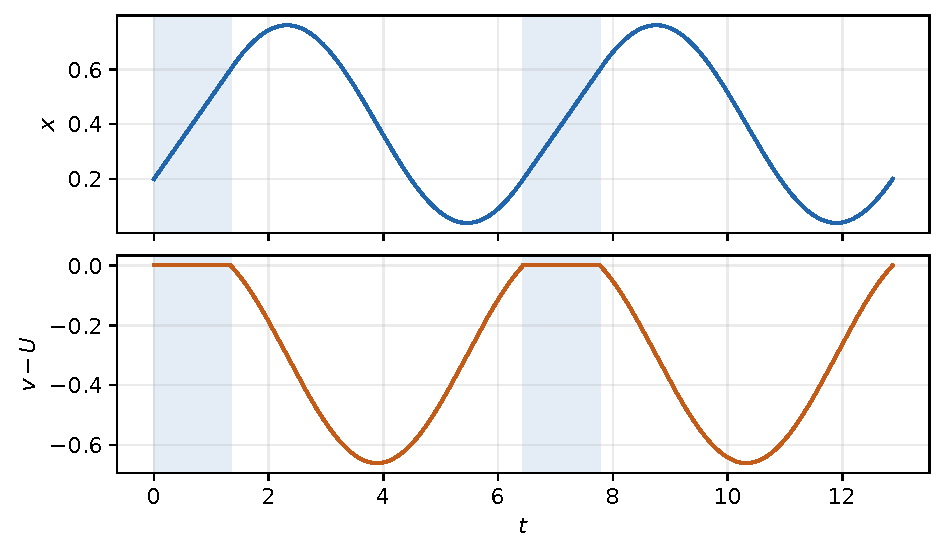
\includegraphics[width=\linewidth]{graphics_v3/stick_slip_cycle.pdf}
\caption{Tapadás és csúszás két egymást követő ciklusban. A kék háttér tapadást jelöl. A laboratóriumi helyzet ekkor változik, a relatív sebesség nulla.}\label{fig:stick_slip_new}
\end{figure}

A kód az egzakt szakaszokat illeszti, így külön ODE-megoldó nélkül ellenőrizhető a váltási logika. Általános gerjesztésnél ugyanezeket a módokat eseményvezérelt integrálással kell összekapcsolni.
\phantomsection\label{use:stick}A teljes MATLAB-program az A függelék \ref{ap:stick}. szakaszában található (\pageref{ap:stick}. oldal).
\exampleend

\section{Zeno-jelenség és tartós kontaktus}\label{sec:zeno}
\subsection{Végtelen sok ütközés véges idő alatt}
A pattogó labda alapmodelljéhez az \cite[1.2. szakasz]{dib}, az ütközések felhalmozódásához és a tapadás kialakulásához a kötet 6.4.3. szakasza ad további hátteret.

Térjünk vissza a labdához. Jelölje $V=\sqrt{2gh_0}$ az első becsapódási sebesség nagyságát, $t_1=V/g$ az első ütközés idejét. Az $n$-edik visszapattanás utáni sebesség $r^nV$, a következő repülés időtartama
\begin{equation}\label{eq:zeno_intervals}
\Delta t_n=\frac{2r^nV}{g},\qquad n=1,2,\ldots.
\end{equation}
Mivel $0<r<1$, a geometriai sor összegezhető:
\begin{equation}\label{eq:zeno_time}
T_Z=t_1+\sum_{n=1}^{\infty}\Delta t_n
=\frac{V}{g}\frac{1+r}{1-r}.
\end{equation}
A $h_0=1\,\mathrm m$, $g=9{,}81\,\mathrm{m/s^2}$, $r=0{,}7$ esetben $T_Z\simeq2{,}55863\,\mathrm s$. Végtelen sok diszkrét esemény történik véges fizikai idő alatt: ez a Zeno-jelenség. A repülési szakaszok száma korlátlanul nő, miközben az állapot $(h,v)=(0,0)$-hoz tart. Ez a modell tulajdonsága, nem integrátorhiba \cite{or_teel}.

\begin{figure}[!htbp]\centering
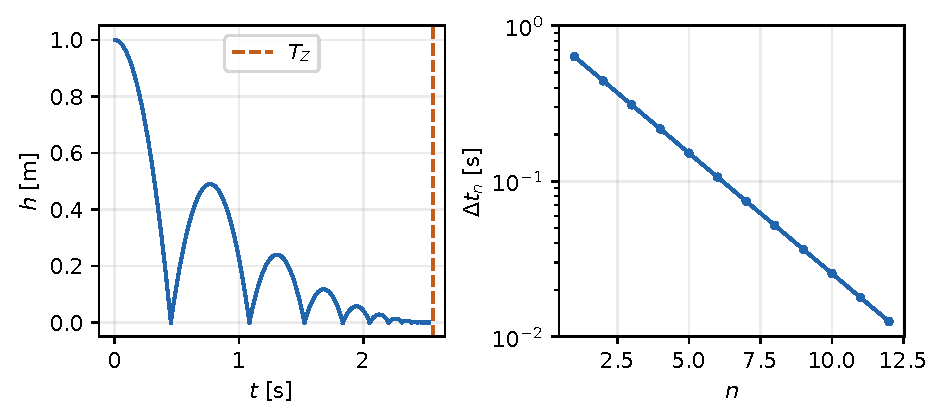
\includegraphics[width=\linewidth]{graphics_v3/zeno_ball.pdf}
\caption{A labda egzakt repülési szakaszai és az ütközési időközök. A jobb oldali logaritmikus skálán a geometriai csökkenés egyenes. Az ábra véges számú szakaszt jelenít meg.}\label{fig:zeno_new}
\end{figure}

A numerikus eseménypattogás ettől eltér: hibás újraindítás vagy kerekítési hiba ugyanazt a gyököt újra és újra megtalálhatja, lényeges időelőrehaladás nélkül. Zeno esetén a pontos repülési időközök is csökkennek. A programunk nyolc ütközés után megáll; nem állítja, hogy addigra a labda fizikailag nyugalomba került.

\subsection{Hogyan folytatjuk a mozgást?}
A szabad esés és a sebesség-reset leképezés önmagában nem ad kontaktuserőt. $T_Z$ után a nyugalomban maradáshoz új módot vezetünk be:
\begin{equation}
h=0,\quad v=0,\quad N=mg,\quad \dot h=\dot v=0,
\end{equation}
ahol $N\geq0$ a talaj nyomóereje. A merev, egyoldali kontaktus feltételei
\begin{equation}\label{eq:contact_complementarity}
h\geq0,\qquad N\geq0,\qquad hN=0.
\end{equation}
Szabad repülésben $N=0$; tartós kontaktusban a kényszert fenntartó erőt számítjuk. Ezek önmagukban nem helyettesítik a becsapódás impulzustörvényét. Általános külső erőnél a kontaktus csak addig tartható fenn, amíg nem igényelne húzó talajerőt; ellenkező esetben elválás történik. A Zeno-idő utáni folytatás tehát kifejezett modellkiegészítés \cite{goebel_sanfelice}.

Ha kis sebességnél numerikusan nyugalomra váltunk, ennek pontossága is becsülhető. Az aktuális visszapattanás utáni $u>0$ sebességtől a még hátralévő repülési idő
\[
T_{\mathrm{marad}}=\frac{2u}{g(1-r)},\qquad
h_{\mathrm{kov}}=\frac{u^2}{2g}.
\]
Egy $u<v_{\mathrm{tol}}$ leállítás legfeljebb $v_{\mathrm{tol}}^2/(2g)$ következő emelkedést hagy el, de a hátralévő idő $r\to1$ esetén nagy lehet. A sebességküszöböt ezért fizikai magasság- és időpontossághoz kell kötni; nem általános gyógyír minden sűrű eseménysorozatra.

\section{Discontinuity-induced bifurcations}\label{sec:boundary_bifs}
A sima bifurkációknál a pálya ugyanazon sima dinamikán belül veszti el stabilitását vagy létezését. Szakaszos rendszernél az is változást okozhat, hogy a pálya eléri a kapcsolási határt. A három itt megkülönböztetett helyzet: egy diszkrét leképezés fixpontjának border-collision bifurcation eseménye, egy folytonos pálya grazing eseménye és egy Filippov sliding szakasz megjelenése. A határ elérése önmagában még nem mondja meg az új pálya stabilitását \cite{champneys_dib}.

\subsection{Border-collision bifurcation egy kétszakaszos leképezésben}
\examplebody

A következő elemi példa a \cite[1.4.3. és 3.4. szakasz]{dib} által tárgyalt folytonos, szakaszonként lineáris leképezések körébe tartozik.

Tekintsük a folytonos, de a határon nem differenciálható modellt:
\begin{equation}\label{eq:border_map}
x_{n+1}=P(x_n;\mu)=
\begin{cases}\mu+\frac12x_n,&x_n\leq0,\\
\mu-\frac32x_n,&x_n>0.
\end{cases}
\end{equation}
$\mu<0$ mellett $x_*=2\mu<0$ stabil fixpont, multiplikátora $1/2$. $\mu=0$-nál eléri a $x=0$ határt. $\mu>0$ mellett a jobb ág fixpontja $x_*=2\mu/5>0$, multiplikátora $-3/2$, tehát instabil. A kétoldali derivált a kritikus pontban nem létezik; nem történt egy sima multiplikátor folyamatos áthaladása a $-1$ értéken.

Keressünk a pozitív paraméteroldalon kétciklust, $x_L<0<x_R$ pontokkal. A két feltétel
\[
x_R=\mu+\tfrac12 x_L,\qquad
x_L=\mu-\tfrac32 x_R
\]
megoldása
\begin{equation}\label{eq:border_two_cycle}
x_L=-\frac{2\mu}{7},\qquad x_R=\frac{6\mu}{7}.
\end{equation}
Az ágfeltételek $\mu>0$ esetén teljesülnek, a kétlépéses multiplikátor $(1/2)(-3/2)=-3/4$, így a ciklus lokálisan aszimptotikusan stabil. A stabil fixpontot a border-collision bifurcation után stabil kétciklus váltja fel. A \ref{fig:border_new}. ábra az egzakt ágakat mutatja; a rövid kód tranziens utáni iterációkkal állítja elő a stabil ágakat. Instabil ágat egyszerű előreiterálással általában nem kapunk meg.

\begin{figure}[!htbp]\centering
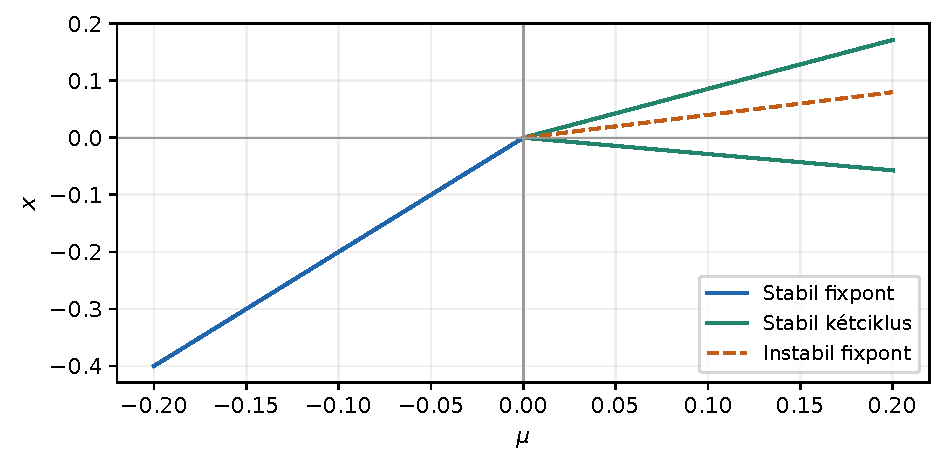
\includegraphics[width=\linewidth]{graphics_v3/border_collision.pdf}
\caption{Border-collision bifurcation $\mu=0$-nál. Folytonos vonal: stabil fixpont, illetve a stabil kétciklus két pontja. Szaggatott vonal: instabil fixpont.}\label{fig:border_new}
\end{figure}
\phantomsection\label{use:border}A teljes MATLAB-program az A függelék \ref{ap:border}. szakaszában található (\pageref{ap:border}. oldal).
\exampleend

\subsection{Grazing és sliding szakasz születése}
\examplebody

A sliding bifurcations osztályozását és a grazing--sliding eset levezetését lásd \cite[8.1. és 8.3.2. szakasz]{dib}.

A 4. fejezet ütköző oszcillátoránál a grazing feltétele $H=0$, $H_xF=0$, $a_H>0$. Ekkor a simán továbbvezetett pálya a kontaktus határát érinti, és a visszatérési leképezésben négyzetgyökös korrekció jelenhet meg. Ez nem azonos a \eqref{eq:border_map} véges meredekségű, szakaszonként lineáris modelljével.

Filippov-rendszerben más mechanizmust látunk. Lokális, dimenziótlan példaként legyen $H=y$, és
\begin{equation}\label{eq:local_sliding_birth}
F_+(x,y)=\begin{pmatrix}1\\x\end{pmatrix}\ (y>0),\qquad
F_-(x,y)=\begin{pmatrix}1\\1\end{pmatrix}\ (y<0).
\end{equation}
A $y=0$, $x<0$ félegyenesen a két mező a felületre mutat, ezért $\dot x=1$, $\dot y=0$ sliding mozgás adódik. A felső sima pályák $dy/dx=x$ alapján
\[
y=\tfrac12x^2+c
\]
parabolák. $c>0$ mellett nincs kontaktus, $c=0$ esetén érintés történik az origóban. $c<0$ esetén a beérkező pálya $x=-\sqrt{-2c}$ pontban eléri a felületet, sliding mozgással jut rajta az origóig, majd elhagyja azt a felső tartomány felé. A sliding szakasz időtartama $\sqrt{-2c}$. Ezzel közvetlenül látható egy sliding szakasz születése.

Itt $c$ a beérkező pályát jelöli, nem a vektormező paramétere. Egy teljes rendszerben a globális visszatérés és egy fizikai paraméter határozhatja meg $c$ értékét. A lokális példa ezért a grazing--sliding mechanizmusát szemlélteti; önmagában nem bizonyít periodikus pályán bekövetkező bifurkációt. A sliding szakasz az ide érkező pályák egy részét ugyanahhoz a kilépő állapothoz vezeti, így a visszatérési leképezés információt veszíthet és nem feltétlenül invertálható \cite{champneys_dib}.

\begin{figure}[!htbp]\centering
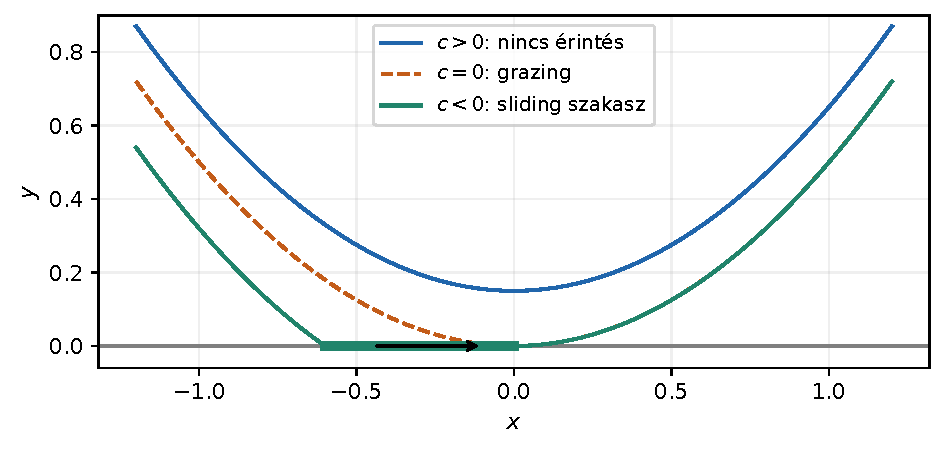
\includegraphics[width=\linewidth]{graphics_v3/sliding_birth.pdf}
\caption{Sliding szakasz megjelenése a lokális példában. A zöld pálya a kapcsolófelületen az origóig halad, majd a felső tartományba lép. A mozgás mindenütt növekvő $x$ irányú.}\label{fig:sliding_birth_new}
\end{figure}
\exampleend

\section{Regularizáció: mikor segít a simítás?}\label{sec:regularization}
\subsection{A simított modell felírása}
Az ideális kapcsolást gyakran folytonos átmenettel helyettesítjük. Egy $H=0$ felület körül például
\begin{equation}
F_\varepsilon=\frac{1+\phi(H/\varepsilon)}2F_+
+\frac{1-\phi(H/\varepsilon)}2F_-,\qquad \phi(s)=\tanh s
\end{equation}
ad sima vektormezőt, ha a két oldali mező is sima a szükséges környezetben. $\varepsilon>0$ az átmenet szélessége, mértékegysége $H$-éval azonos. A regularizáció kapcsolatot teremt a sima és a Filippov-leírás között, de a megoldások és bifurkációk egyezése további feltételeket igényel \cite{sotomayor_teixeira}.

\subsection{Amikor segít: egy csúszó test lefékeződése}
\examplebody

Legyen a tömeg és a Coulomb-súrlódási erő dimenziótlanul egy, külső erő ne hasson, a kezdeti sebesség pedig $v(0)=1$. A test mozgás közben állandóan lassul, megállás után pedig nyugalomban marad. Az ideális Filippov-modell és megoldása:
\[
\dot v\in-\operatorname{Sign}(v),\qquad
v(t)=\max(1-t,0),\quad t\geq0,
\]
ahol $\operatorname{Sign}(v)=\{\operatorname{sign}(v)\}$, ha $v\neq0$, és $\operatorname{Sign}(0)=[-1,1]$. A megállás időpontja $t=1$.

A simítás ugyanennek az egyszerű modellnek a jobb oldalát teszi folytonossá:
\[
\dot v_\varepsilon=-\tanh(v_\varepsilon/\varepsilon),\qquad
v_\varepsilon(0)=1.
\]
Így egy szokásos sima ODE-megoldóval, külön megállási esemény és módváltás nélkül számíthatjuk a lassulást. A példát kézzel is ellenőrizhetjük: $z=\sinh(v_\varepsilon/\varepsilon)$ bevezetésével $\dot z=-z/\varepsilon$, tehát
\begin{equation}\label{eq:regularization_braking_exact}
v_\varepsilon(t)=\varepsilon\operatorname{arsinh}
\left[\sinh(1/\varepsilon)e^{-t/\varepsilon}\right].
\end{equation}
A simított sebesség pozitív marad, és monoton nullához tart. Az ideális sebességtől vett eltérés $0\leq t\leq1$ között nő, utána csökken; maximuma ezért $t=1$-nél van:
\[
0\leq v_\varepsilon(t)-\max(1-t,0)
\leq\varepsilon\operatorname{arsinh}\!\left(\frac{1-e^{-2/\varepsilon}}2\right)
<0{,}482\varepsilon.
\]
Például $\varepsilon=0{,}01$ mellett a sebességhiba \emph{minden} $t\geq0$ időpontban kisebb $0{,}00482$-nél, a nyugalmi határállapot pedig helyes. Ha a kérdés a sebesség lefutása adott pontossággal, a regularizáció itt jól használható, és a hiba $\varepsilon$ csökkentésével kontrollálható. A pontos, véges idejű megállást azonban nem őrzi meg: ehhez továbbra is az ideális eseménykezelés szükséges. A kis $\varepsilon$ miatti rövid relaxációs időt a numerikus megoldónak fel kell oldania.

A \ref{fig:regularization_braking}. ábra a numerikus simított megoldásokat az ideális sebességgel hasonlítja össze. Az alsó panel a megállás környéki hibát nagyítja ki: a legnagyobb eltérés $t=1$-nél jelentkezik, és $\varepsilon$ csökkentésével arányosan mérséklődik. A teljes, mindkét példát előállító MATLAB-kód az A függelék \ref{ap:regularization}. szakaszában található.
\begin{figure}[htbp]\centering
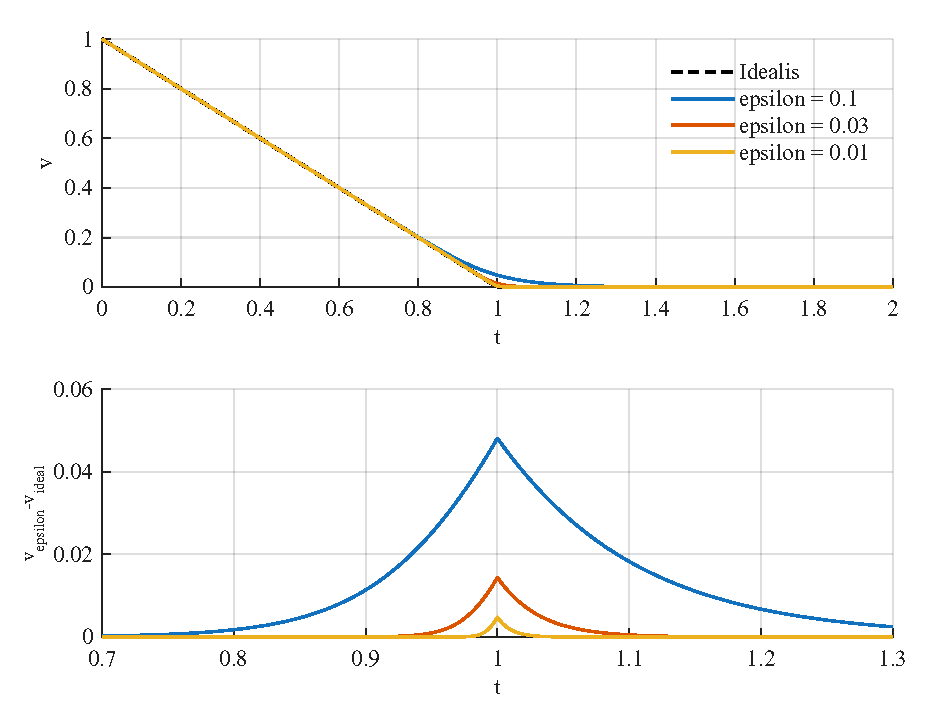
\includegraphics{graphics_v3/regularization_braking.pdf}
\caption{Lefékeződés külső erő nélkül, $v(0)=1$. Fent: az ideális és a három simított sebesség; lent: a sebességhiba a megállás környezetében. A simított görbék nullához tartanak, de nem érik el véges idő alatt.}\label{fig:regularization_braking}
\end{figure}
\exampleend

\subsection{Amikor félrevezet: tapadás helyett tartós kúszás}
\examplebody

Most ugyanarra az egységnyi tömegre hasson a súrlódási határnál kisebb, állandó $q=1/2$ erő, és induljunk nyugalomból: $x(0)=v(0)=0$. A kérdés az, hogy a test helyben marad-e. Az ideális modellben a statikus súrlódás kiegyenlíti az erőt, ezért $v(t)=0$, $x(t)=0$ minden időben. A simított modell más választ ad.

Az eltérés általános $q$ terhelésre is egyszerűen leírható. A dimenziótlan $m=F=1$, $0<q<1$ esetben az ideális statikus súrlódás $v=0$ mellett kiegyenlítheti a terhelést. A simított egyenlet viszont
\begin{equation}\label{eq:regularized_friction}
\dot v=q-\tanh(v/\varepsilon).
\end{equation}
A $v=0$ állapotban $\dot v=q>0$, tehát nincs pontos tapadás. Az egyetlen stacionárius sebesség
\begin{equation}\label{eq:creep_speed}
v_\varepsilon=\varepsilon\operatorname{artanh}(q),\qquad
\left.\frac{d\dot v}{dv}\right|_{v_\varepsilon}
=-\frac{1-q^2}{\varepsilon}<0.
\end{equation}
A sebesség stabil, de pozitív: a test lassan kúszik. $q=1/2$ mellett $v_\varepsilon\simeq0{,}549306\varepsilon$. Rögzített véges időn a kúszás hatása csökkenhet $\varepsilon$-nal, de hosszú idő alatt jelentős helyzethiba gyűlhet össze. A határerőhöz közeli $q\to1^-$ tartományban ez a becslés nem egyenletes.

A $q=1/2$, $\varepsilon=0{,}01$ példában a beálló sebesség mindössze $v_\varepsilon\simeq0{,}00549306$, de folyamatosan pozitív. A rövid kezdeti beállás után
\[
x_\varepsilon(t)\simeq0{,}00549306\,t,
\]
így $t=100$-nál már körülbelül $0{,}549$ a helyzeteltérés, míg az ideális test továbbra is az origóban áll. Az ODE pontosabb integrálása ezt nem szünteti meg: a kúszás a simított egyenlet megoldásának tulajdonsága.

Az $\varepsilon$ csökkentése a hibát lassabban felhalmozódóvá teszi, de véges $\varepsilon$ mellett nem állítja vissza a tapadást. Például $\varepsilon=0{,}001$ és $t=1000$ mellett közel ugyanekkora elmozdulást kapunk. Általánosan $t=1/\varepsilon$ időskálán $x_\varepsilon(t)\to\operatorname{artanh}(1/2)\simeq0{,}549306$, miközben az ideális elmozdulás nulla. A közelítés tehát rögzített véges időn javulhat, de tetszőlegesen hosszú időre nem ad egyenletesen kis helyzethibát.

Ha a feladat a tapadás fennmaradásának vagy a hosszú idejű helyzetnek a meghatározása, ez a simítás nem megfelelő modell. Ilyenkor külön tapadási módot használunk a $|q|\leq1$ erőfeltétellel, és csak a határ túllépésekor indítjuk el a mechanikai csúszást. A két példa különbsége az ellenőrzött mennyiségben is megmutatkozik: a kis sebességhiba még nem garantál kis, hosszú idejű helyzethibát.


A \ref{fig:regularization_creep}. ábrán felül a pozitív kúszósebesség gyors beállását, alul a hosszú idő alatt felhalmozódó elmozdulást látjuk. Az ideális megoldás mindkét panelen nulla. A két panel időtengelye eltér: a sebességnél $0\leq t\leq1$, a helyzetnél $0\leq t\leq100$ szerepel, hogy a gyors beállás és a lassú hibafelhalmozódás egyaránt látható legyen. A teljes kód az A függelék \ref{ap:regularization}. szakaszában található.
\begin{figure}[htbp]\centering
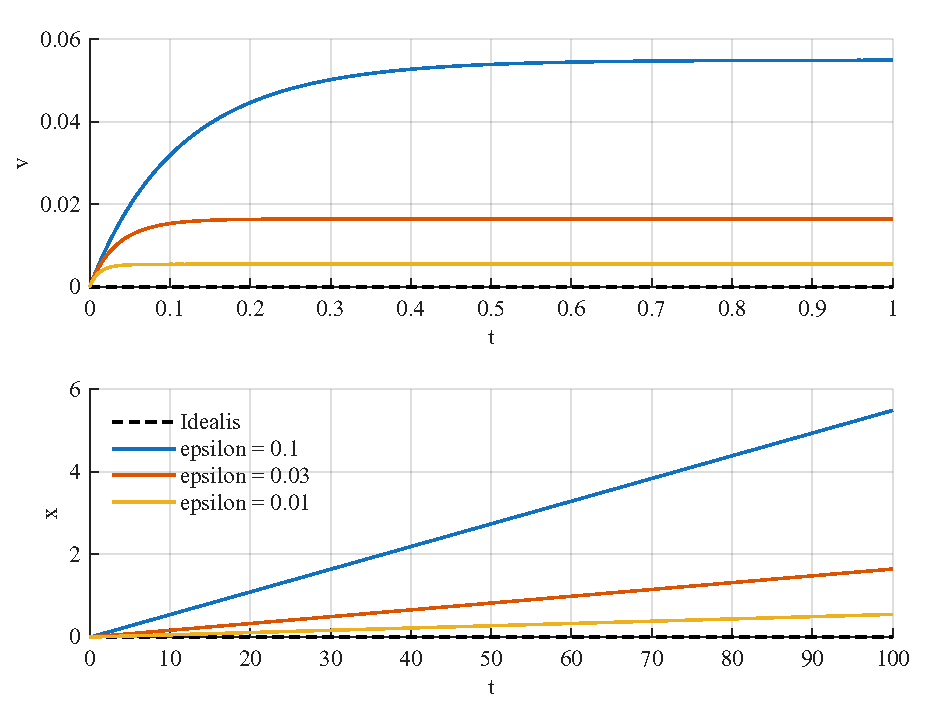
\includegraphics{graphics_v3/regularization_creep.pdf}
\caption{Tapadás helyett kúszás: $q=1/2$, $x(0)=v(0)=0$. Fent a sebesség, lent az elmozdulás összehasonlítása. A kisebb simítási szélesség kisebb sebességet ad, de véges $\varepsilon$ mellett az elmozdulás tovább növekszik.}\label{fig:regularization_creep}
\end{figure}

\begin{figure}[!htbp]\centering
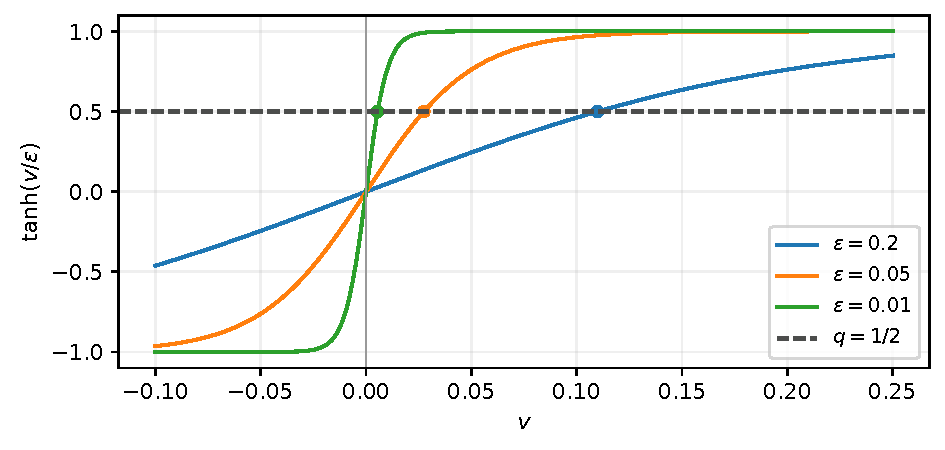
\includegraphics[width=\linewidth]{graphics_v3/friction_regularization.pdf}
\caption{Simított súrlódás $q=1/2$ mellett. A terhelés és a súrlódási görbe metszése pozitív kúszósebességet ad; az ideális tapadás sebessége nulla.}\label{fig:regularization_new}
\end{figure}
\phantomsection\label{use:regularization}A teljes MATLAB-program az A függelék \ref{ap:regularization}. szakaszában található (\pageref{ap:regularization}. oldal).

A kód a kis $\varepsilon$ mellett gyors relaxáció miatt \texttt{ode15s} megoldót használ. A relaxáció időskálája $\varepsilon/(1-q^2)$. Összetettebb modellben ez a lassú mechanikai időskálához képest numerikus merevséget okozhat. A simítás szélessége modellparaméter; a megoldó toleranciája ettől külön numerikus paraméter. Először rögzített $\varepsilon$ mellett kell numerikus konvergenciát vizsgálni, majd több $\varepsilon$ értékkel a modellérzékenységet.
\exampleend

\subsection{Merev fal helyett rugalmas kontaktus}
\examplebody

A másik gyakori közelítés az azonnali ütközés helyett rövid kontaktusfázis. Legyen $h$ a rés, $\delta=\max(0,-h)$ a benyomódás. A legegyszerűbb tisztán rugalmas büntetőmodell $N=K\delta$ nyomóerőt ad. A kontaktus közbeni kis behatolás ekkor a modell része, a kontaktus időskálája $\sqrt{m/K}$.

Külső erők nélkül a benyomódásra $m\ddot\delta+K\delta=0$ adódik. $\delta(0)=0$, $\dot\delta(0)=V>0$ mellett
\[
\delta(t)=\frac{V}{\sqrt{K/m}}\sin\!\left(\sqrt{K/m}\,t\right).
\]
Az első visszatérés ideje $t_c=\pi\sqrt{m/K}$, a maximális behatolás $V\sqrt{m/K}$. Kilépéskor a sebesség nagysága ismét $V$: ez $r=1$ visszapattanásnak felel meg. A nagyobb $K$ rövidebb kontaktust és kisebb behatolást ad, de \emph{önmagában nem hoz létre} $r<1$ energiaveszteséget. Ehhez disszipatív kontaktustörvény és elválási feltétel kell; az így kapott visszapattanási tényezőt a választott törvényből kell meghatározni.

Az ideális ütköző, a rugalmas kontaktus és a simított kapcsolás különböző modellek. Összevetésükkor az ütközési impulzust, a visszapattanási sebességet, a kontaktusidőt és a periódust érdemes ellenőrizni. Különösen grazing vagy tartós kontaktus közelében nem elegendő arra hivatkozni, hogy az átmenet keskeny vagy a rugó merev: a közelítés éppen a vizsgált helyi dinamikát változtathatja meg.
\exampleend

\section{Boundary equilibrium bifurcations}\label{sec:beb}
Egy paraméter változtatásakor az egyensúly elérheti a kapcsolófelületet. Ezt a helyzetet \emph{boundary equilibrium bifurcation} (BEB) néven tárgyalja \cite[5.1--5.2. szakasz]{dib}. Először a két oldali vektormező egyensúlyait külön számítjuk ki, majd ellenőrizzük, hogy a kapott gyök a megfelelő tartományban van-e. Az ilyen gyök \emph{admissible equilibrium}; a másik tartományba eső, formálisan folytatott gyök \emph{virtual equilibrium}. A kapcsolófelületen fekvő egyensúly \emph{boundary equilibrium}. A virtual equilibrium nem a teljes rendszer állandósult megoldása.

\subsection{Persistence: az egyensúly fennmarad}
\examplebody

Egy erősen csillapított, kétféle pozitív merevségű rugóval megtámasztott szerkezet dimenziótlan modellje legyen
\begin{equation}
 \dot x=\begin{cases}\mu-x,&x<0,\\ \mu-2x,&x\geq0.\end{cases}
 \label{eq:beb_persistence}
\end{equation}
Itt $x$ az elmozdulás, $\mu$ az állandó terhelés. A vektormező $x=0$-ban folytonos. A bal oldali egyensúlyjelölt $x_L=\mu$, a jobb oldali $x_R=\mu/2$. Ha $\mu<0$, csak $x_L$ admissible; ha $\mu>0$, csak $x_R$ admissible. A fizikai egyensúly tehát
\[
 x^*(\mu)=\begin{cases}\mu,&\mu\leq0,\\\mu/2,&\mu\geq0.\end{cases}
\]
Mindkét oldalon aszimptotikusan stabil, mert az állapot szerinti derivált rendre $-1$ és $-2$. A kritikus pontban is minden közeli pálya az origóhoz tart. Ezt az ággeometriát \emph{persistence} esetnek nevezzük: a megoldás átjut a kapcsolófelületen, de stabilitása itt nem változik. Az egyensúlyág meredekségének törése önmagában nem jelent új rezgésállapotot vagy stabilitásvesztést.
\exampleend

\subsection{Non-smooth fold: két egyensúly eltűnik}
\examplebody

A jobb oldalon aktív szabályozással negatív eredő merevséget is létrehozhatunk. Ennek legegyszerűbb helyi modellje
\begin{equation}
 \dot x=\begin{cases}\mu-x,&x<0,\\\mu+x,&x\geq0.\end{cases}
 \label{eq:beb_fold}
\end{equation}
Ez is folytonos $x=0$-ban. Ha $\mu<0$, az $x_L=\mu<0$ egyensúly stabil, az $x_R=-\mu>0$ egyensúly instabil. Ha $\mu>0$, mindkét jelölt virtual, ezért a teljes rendszernek nincs egyensúlya. A két admissible ág $\mu=0$-nál találkozik és eltűnik: ez a \emph{non-smooth fold}. A kritikus egyensúly balról vonzó, jobbról taszító, tehát kétoldali értelemben nem stabil. A pozitív oldali $+x$ tag nem passzív rugót, hanem destabilizáló visszacsatolást modellez. Az egyensúly megszűnése ebből a helyi modellből nem igazolja periodikus pálya létrejöttét.
\exampleend

\subsection{Filippov-példa: valódi egyensúlyból pseudo-equilibrium}
\examplebody

Legyen $H(x,y)=y$, és tekintsük az alábbi dimenziótlan, relés beavatkozást szemléltető modellt:
\begin{equation}
 F^+(x,y)=\begin{pmatrix}-x\\\mu-y\end{pmatrix}\quad(y>0),\qquad
 F^-(x,y)=\begin{pmatrix}-x\\1\end{pmatrix}\quad(y<0).
 \label{eq:beb_filippov}
\end{equation}
Az $x$ változó egy stabil belső állapot, $y$ a szabályozott eltérés. Negatív eltérésnél a beavatkozás állandó pozitív változási sebességet hoz létre; pozitív eltérésnél az eltérés $\mu$ felé relaxál. Ha $\mu>0$, a $(0,\mu)$ egyensúly admissible és stabil. A felületi normális komponensek $\mu$ és $1$, ezért ekkor nincs attracting sliding.

Ha $\mu<0$, a felső mező egyensúlya virtual lesz, viszont $\mu<0<1$ miatt a két mező a felület felé mutat. A Filippov-kombinációban
\[
 F_s=(1-\alpha)F^++\alpha F^-,\qquad
 \alpha=\frac{-\mu}{1-\mu}\in(0,1),\qquad F_s(x,0)=\begin{pmatrix}-x\\0\end{pmatrix}.
\]
Így $(0,0)$ stabil \emph{pseudo-equilibrium}: a sliding dinamika egyensúlya, jóllehet egyik oldali mező sem nulla ott. A felület vonzó, és azon $\dot x=-x$ biztosítja a tangenciális stabilitást. A $\mu=0$ kritikus pontban az admissible egyensúly a felületre ér; $\mu<0$ esetén a stabil állandósult állapot sliding formájában folytatódik. A konvex súly tartományának ellenőrzése lényeges: $\mu>0$ esetén a formális képlet nem ad megengedett sliding megoldást. A Filippov-féle BEB további eseteit \cite[5.2. szakasz]{dib} rendszerezi.

\begin{figure}[!htbp]\centering
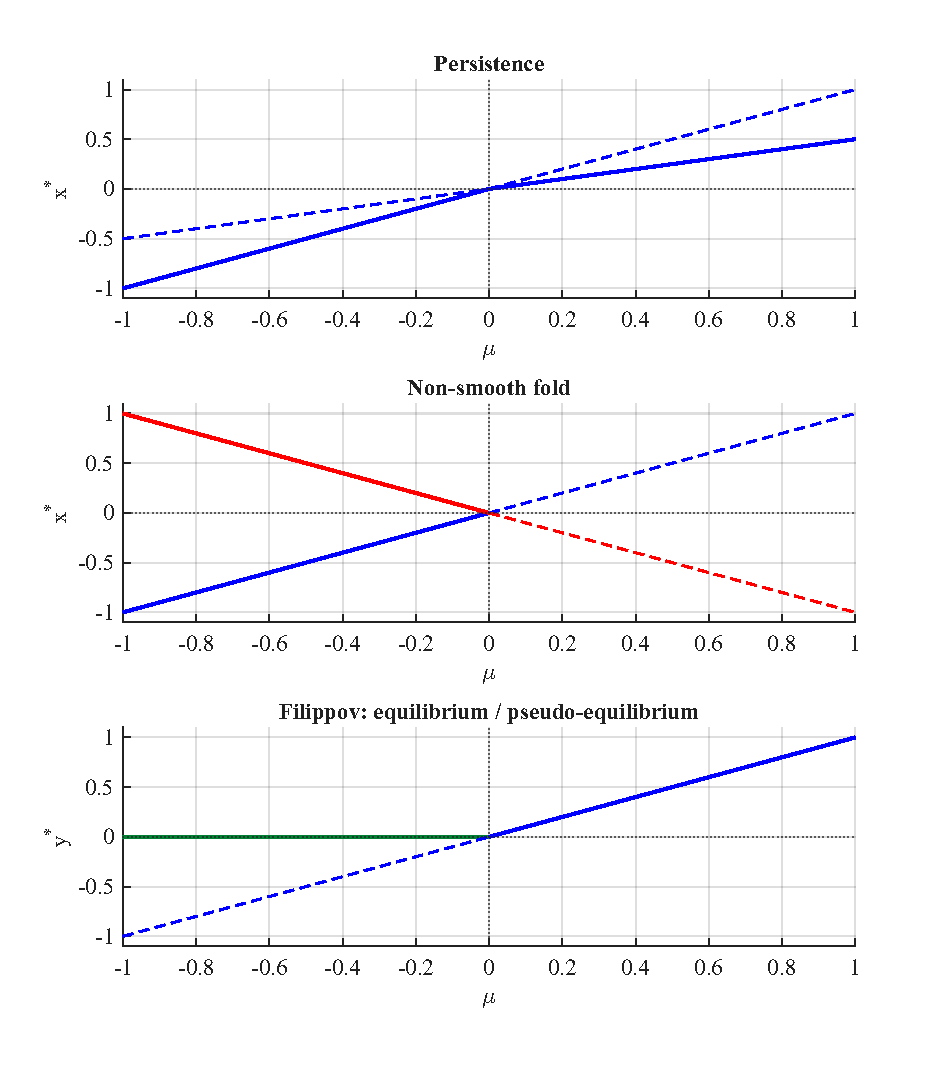
\includegraphics{graphics_v3/boundary_equilibria.pdf}
\caption{Három egyszerű BEB-példa. A folytonos vonal admissible, a szaggatott virtual ágat jelöl. A kék ág stabil, a piros instabil. Az alsó panelen a zöld ág stabil pseudo-equilibrium: a kapcsolófelületen folytatja a stabil állandósult állapotot. A színezés csak az admissible ágak fizikai stabilitását állítja.}\label{fig:beb_examples}
\end{figure}
\phantomsection\label{use:beb}A teljes ábrageneráló MATLAB-program az A függelék \ref{ap:beb}. szakaszában található.
\exampleend

\section{A sliding bifurcations négy helyi típusa}\label{sec:four_sliding}
A kapcsolófelület elérése és a sliding region határának elérése eltérő esemény. Az utóbbinál valamelyik oldali mező normális komponense nulla. A négy alaphelyzetet \cite[8.1. szakasz]{dib} tárgyalja; relés szabályozási alkalmazást a könyv 8.2. szakasza ad. Az alábbi dimenziótlan modellek a helyi pályageometriát szemléltetik. A pályacsalád változtatása önmagában még nem periodikus pálya bifurkációja: ehhez olyan globális visszatérés is kell, amely a pályát újra ebbe a környezetbe vezeti.

\subsection{Crossing--sliding}
\examplebody

Legyen $H(x,y)=y$, felül $F^+=(1,x)^T$, alul $F^-=(1,1)^T$. A $y=0$, $x<0$ félegyenes attracting sliding region, mert a normális komponensek $x<0<1$. Mindkét mező első komponense egy, ezért a sliding mozgás $\dot x=1$, $\dot y=0$. A pálya a határon, $x=0$-nál a felső tartományba lép ki.

Érkezzen egy alsó pálya a felület $(s,0)$ pontjába. Ha $s>0$, áthalad a felületen, majd a felső pálya $y=(x^2-s^2)/2$. Ha $s<0$, előbb sliding mozgással halad az $s\leq x\leq0$ szakaszon, és csak ezután követi a $y=x^2/2$ parabolát. Az $s=0$ kritikus esetben az érkező mező normális sebessége továbbra is $1$: az érkezés nem grazing. A változás a rövid sliding szakasz megjelenése. Mérnöki értelemben egy relés átkapcsolás után itt kezdődhet tartós, ideális sliding üzem.
\exampleend

\subsection{Grazing--sliding}
\examplebody

Ugyanebben a mezőben most a felső tartományból érkezzünk a $y=x^2/2+c$ pályán. Ha $c>0$, a pálya nem éri el a felületet. Ha $c=0$, az origóban érinti, és $\dot y=0$, $\ddot y=1$: ez nemelfajuló grazing. Ha $c<0$, az első találkozás $x=-\sqrt{-2c}$-nél történik, majd a pálya sliding mozgással jut az origóba. A sliding szakasz hossza $\sqrt{-2c}$. Itt tehát egy addig kapcsolásmentes mozgás válik sliding szakaszt tartalmazóvá. Száraz súrlódásnál ez egy új tapadási szakasz megjelenésének helyi modellje lehet; az adott súrlódási rendszerben a normális irányt a relatív sebesség határozza meg.
\exampleend

\subsection{Switching--sliding}
\examplebody

Most legyen $F^+=(1,-x)^T$, $F^-=(1,1)^T$. Az attracting sliding region $x>0$, és rajta továbbra is $\dot x=1$: a sliding mozgás a határtól távolodik. Egy alsó pálya ismét $(s,0)$-ban érkezzen. Ha $s>0$, azonnal sliding indul. Ha $s<0$, a pálya előbb a felső tartományba lép, ahol
\[
 y=\frac{s^2-x^2}{2},\qquad s\leq x\leq-s,
\]
majd $x=-s>0$-nél újra eléri a felületet és sliding mozgásra vált. Mindkét esetben van sliding, de az egyikben ezt rövid szabad mozgási szakasz előzi meg. A lényeg a kapcsolási sorrend megváltozása, nem az első sliding szakasz létrejötte.
\exampleend

\subsection{Adding--sliding}
\examplebody

A sliding pálya magának a sliding regionnak a határát is érintheti. Ennek természetes geometriájához két tangenciális koordinátát használunk. Legyen az állapot $(s,z,y)$, $H=y$, továbbá
\begin{equation}
 F^+=\begin{pmatrix}1\\0\\z-s^2\end{pmatrix},\qquad
 F^-=\begin{pmatrix}1\\0\\1\end{pmatrix}.
 \label{eq:adding_local}
\end{equation}
Az attracting sliding region $y=0$, $z<s^2$; a sliding mozgás $\dot s=1$, $\dot z=0$. A $z=\mu$ szinten haladó családban $\mu<0$ esetén megszakítás nélküli sliding zajlik. A $\mu=0$ pálya az origóban érinti a sliding region parabola alakú határát. Ha $\mu>0$, a pálya $s=-\sqrt\mu$-nél elhagyja a felületet. A szabad szakaszon
\begin{equation}
 y(s)=\mu s-\frac{s^3}{3}+\frac23\mu^{3/2},\qquad
 -\sqrt\mu\leq s\leq2\sqrt\mu.
\end{equation}
Ezt a $dy/ds=\mu-s^2$ egyenlet integrálásával, $y(-\sqrt\mu)=0$ feltétellel kapjuk. A visszaérkezés $s=2\sqrt\mu$-nél történik; ott $F_y^+=-3\mu<0$, így ismét sliding indul. Egy korábbi sliding intervallum helyén két sliding intervallum és köztük egy szabad kitérés jelenik meg. A maximális eltérés $4\mu^{3/2}/3$. Itt $\mu$ a pályacsalád állandó $z$ koordinátája; egy teljes rendszerben a globális dinamika határozná meg, hogyan függ ez a fizikai vezérlőparamétertől. Relés szabályozásnál ez egy rövid kilépés lehet a sliding üzemből.

\begin{figure}[!htbp]\centering
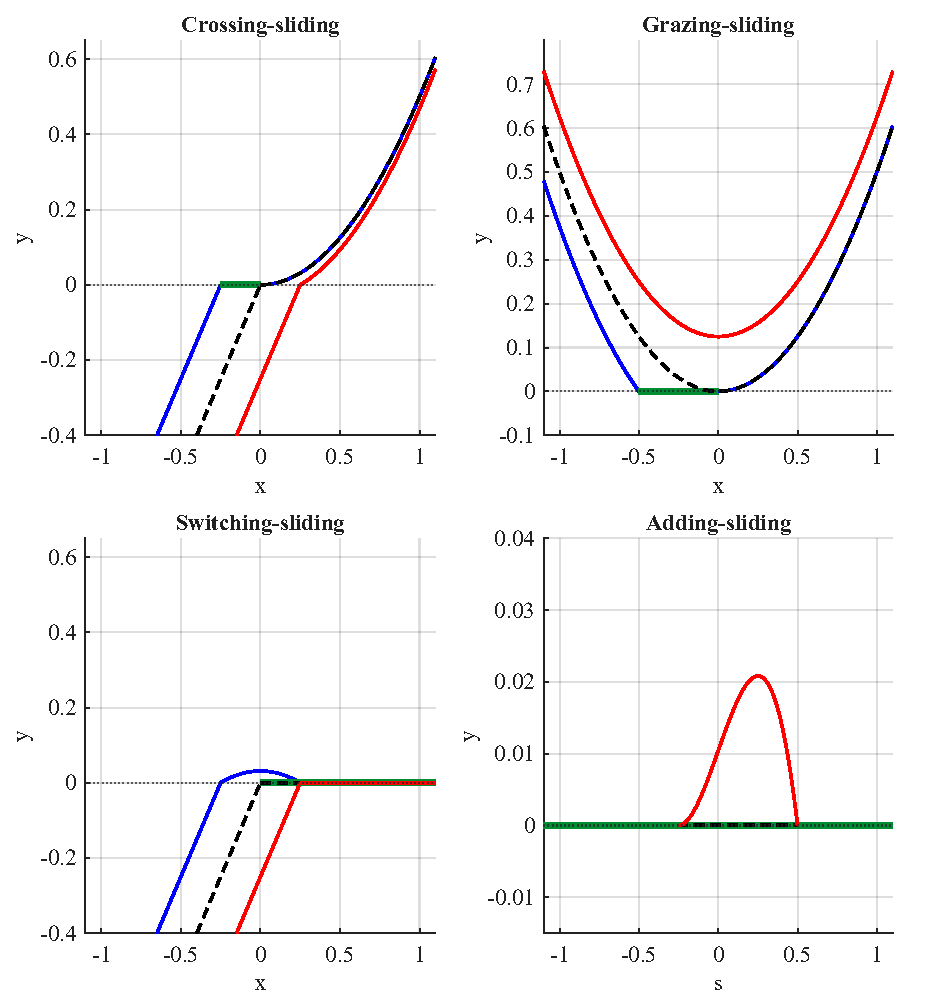
\includegraphics{graphics_v3/sliding_geometries.pdf}
\caption{A négy sliding geometria egzakt helyi pályákon. A kék, fekete szaggatott és piros görbe a kritikus helyzet két oldalát, illetve a kritikus pályát mutatja; a vastag zöld részek sliding szakaszok. Az adding--sliding panel a háromdimenziós pályák $(s,y)$ vetülete, így a megszakítás nélküli sliding pályák egymásra vetülnek. Minden panelen balról jobbra halad az idő.}\label{fig:four_sliding}
\end{figure}
\phantomsection\label{use:sliding_types}Az egzakt pályákat kirajzoló teljes MATLAB-kód az A függelék \ref{ap:sliding_types}. szakaszában szerepel.
\exampleend

\section{Grazing folytonos piecewise-smooth rendszerben}\label{sec:continuous_grazing}
Az ütközéses rendszer grazing leképezésének square-root tagját nem szabad automatikusan átvinni egy folytonos vektormezőre. Ha a kapcsolófelületen maga a vektormező folytonos, de a deriváltja ugrik, a nemelfajuló grazing tipikus helyi korrekciója $3/2$ rendű. Ennek feltételeit és a discontinuity mapping levezetését \cite[7.2. szakasz, különösen 7.1. tétel]{dib} adja meg.

\subsection{Egyszerű mechanikai modell: egyoldali rugó}
\examplebody

Egy $m$ tömegre a kontaktustól elfelé ható állandó $ma$ erő működik, ahol $a>0$. A rés legyen $h$, sebessége $v$; a $h<0$ tartományban egy $k$ merevségű rugó kapcsolódik be. A modell
\begin{equation}
 \dot h=v,\qquad \dot v=a-\kappa\min(h,0),\qquad \kappa=k/m>0.
 \label{eq:continuous_contact}
\end{equation}
A negatív $h$ itt rugalmas benyomódás, a modell megengedett állapota. Nincs sebességugrás vagy reset. A mező $h=0$-ban folytonos, Jacobi-mátrixa viszont a két oldalon
\[
 A_+=\begin{pmatrix}0&1\\0&0\end{pmatrix},\qquad
 A_-=\begin{pmatrix}0&1\\-\kappa&0\end{pmatrix}.
\]
A grazing állapot $(h,v)=(0,0)$: ott $\dot h=0$, de $\ddot h=a>0$.


A rugó nélküli referencia $h_0(t)=-\varepsilon+at^2/2$, ahol $\varepsilon>0$ a referencia behatolási mélysége. A belépési sebesség nagysága $V=\sqrt{2a\varepsilon}$, a referencia két felületi metszése közti idő $T_0=2V/a$. A belépéstől mért $\tau$ idővel a valódi kontaktuspálya
\begin{equation}
 h_c(\tau)=\frac a\kappa(1-\cos\sqrt\kappa\tau)
 -\frac V{\sqrt\kappa}\sin\sqrt\kappa\tau.
\end{equation}
Az első pozitív zérus és a hozzá tartozó sebesség
\[
 T_c=\frac2{\sqrt\kappa}\arctan\frac{V\sqrt\kappa}{a},\qquad v_c(T_c)=V.
\]
A két kilépési sebesség egyaránt $V$, de a kilépés időpontja eltér! Ezért az állapotokat közös időre kell hozni. A valódi pálya hamarabb hagyja el a kontaktust, majd $d=T_0-T_c>0$ ideig ismét $\dot v=a$ szerint mozog. A referencia kilépési időpontjában a különbség pontosan
\begin{equation}
 \Delta v=ad,\qquad \Delta h=Vd+\frac12ad^2.
 \label{eq:continuous_grazing_exact}
\end{equation}
Az $\arctan u=u-u^3/3+O(u^5)$ sorfejtést behelyettesítve
\begin{equation}
 \Delta v=\frac{4\kappa}{3}\sqrt{\frac2a}\,\varepsilon^{3/2}
 +O(\varepsilon^{5/2}),\qquad
 \Delta h=\frac{8\kappa}{3a}\varepsilon^2+O(\varepsilon^3).
 \label{eq:continuous_grazing_order}
\end{equation}
Az esemény időtartama $O(\sqrt\varepsilon)$, de ezalatt a két mező gyorsuláskülönbsége csak $O(\varepsilon)$. Szorzatuk adja a vezető $O(\varepsilon^{3/2})$ sebességkorrekciót. A pozíciókomponens ebben a modellben még magasabb rendű. A vezető tag együtthatójának dimenziója is helyes: $[\kappa]=\mathrm{s}^{-2}$ és $[a]=\mathrm{m}\,\mathrm{s}^{-2}$ mellett $\kappa a^{-1/2}\varepsilon^{3/2}$ sebesség.

Ha a referencia nem hatol be, nincs kontaktuskorrekció. Ezért a paraméterfüggésben egyoldali $[\varepsilon]_+^{3/2}$ jellegű tag jelenik meg. Ennek első deriváltja a kritikus pontban nulla, míg második deriváltja a pozitív oldalról korlátlan. Ez lényegesen enyhébb szingularitás, mint a merev ütközésnél fellépő square-root tag. Az eredmény rögzített véges $\kappa$ és kis $\varepsilon$ mellett érvényes; a $\kappa\to\infty$ merev kontaktushatár nem helyettesíthető be ebbe a sorfejtésbe. Periodikus pálya bifurkációjának megállapításához itt is szükséges a teljes visszatérési leképezés.

\begin{figure}[!htbp]\centering
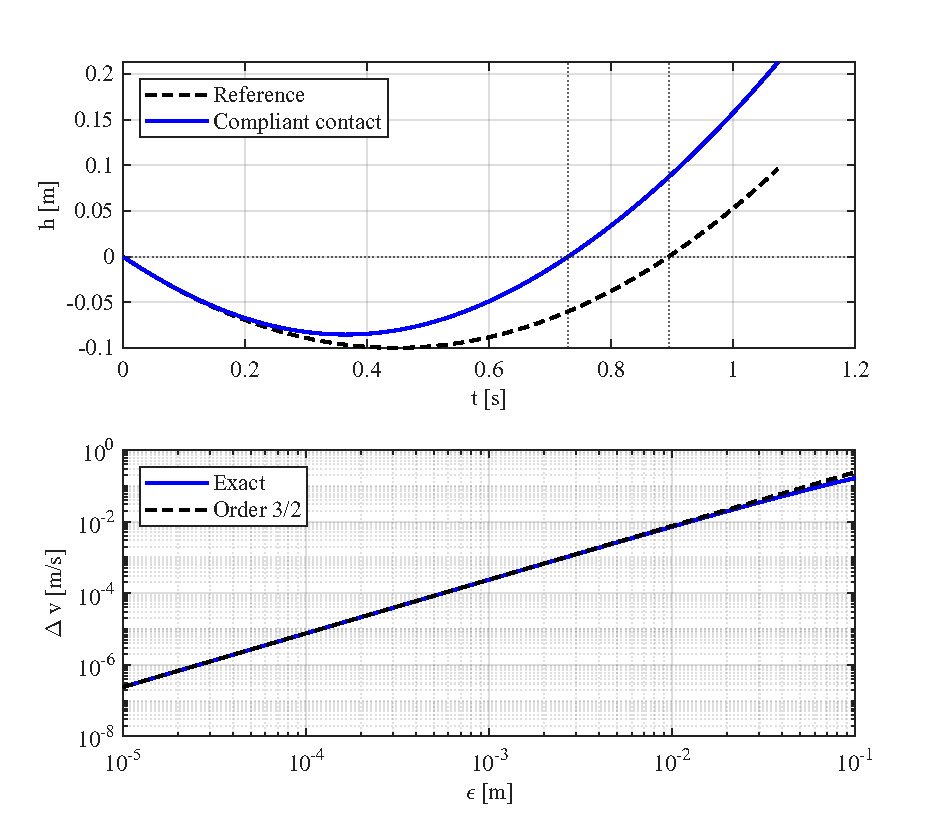
\includegraphics{graphics_v3/continuous_grazing.pdf}
\caption{Folytonos kontaktusmodell, $a=1\,\mathrm{m/s^2}$, $\kappa=4\,\mathrm{s^{-2}}$. Felül a referencia és a rugós pálya résfüggvénye $\varepsilon=0.1\,\mathrm m$ esetén; az idő a belépéstől indul. A rugó csökkenti a benyomódást és előrehozza a kilépést. Alul az azonos időpontban mért egzakt sebességkorrekció és annak $3/2$ rendű közelítése logaritmikus tengelyeken.}\label{fig:continuous_grazing}
\end{figure}
\FloatBarrier
\phantomsection\label{use:continuous_grazing}A teljes MATLAB-program az A függelék \ref{ap:continuous_grazing}. szakaszában található; az egzakt megoldást és a rendbecslést is kiértékeli.
\exampleend

